% =====================================================================
%  chunks/appb.tex —— 原书 p.283–291（PDF 290–298）
%  附录：3 维流形与纽结拓扑学的新进展
%  §2 纽结（下）：Jones 型多项式；§3 Vassiliev 不变量
% =====================================================================

% [原文 p.283]
生成元 $\sigma_i$ 由它在 $V_i\otimes V_{i+1}$ 上的「局部」作用所决定（因为它在其余一切因子上都恒等作用），而「平移不变」是说：对一切 $i$，$\rho(\sigma_i)$ 的作用方式与 $S$ 在 $V\otimes V$ 上的作用相同。

（很容易设想这一构造的种种变体，即用 $\Z$ 的不同的（周期）划分；但迄今为止尚未找到有趣的例子。）

\begin{quote}
\itshape
一个表示 $\rho$ 称为具有 Markov 性质，如果存在一个与 $n$ 无关的常数 $A$，使得对每个 $n$ 与每个辫 $a\in B_n$，都有
\[
\Tr[\rho_n(a)]A=\Tr[\rho_{n+1}(a\sigma_{n+1})].
\]
\end{quote}

% [Tutor Note: Markov 性质的要害是：把辫闭合成链环时取迹所得的量的稳定化行为受控——右乘 $\sigma_{n+1}^{\pm 1}$ 只差常数因子 $A^{\pm 1}$；而乘上 $A^{-w(a)}$（$w(a)$ 为辫的字长指数和）正是为了抵消第一种 Reidemeister 变换带来的因子，于是 $A^{-w(a)}\Tr[\rho_n(a)]$ 才是链环的拓扑不变量。此处 $A$ 是一个由具体表示确定的稳定化常数，后文诸例中它会与括号多项式的变量同形，读者须按语境区分。]

于是按 Jones 的结果，给定这样的表示 $\rho$，量
\[
A^{-w(a)}\Tr[\rho_n(a)],\qquad
a=\sigma_{i_1}^{j_1}\cdots\sigma_{i_m}^{j_m}\in B_n,
\]
其中 $w(a)=\sum_{k=1}^{m}j_k$，给出一个拓扑不变量。

下面将给出这样的表示的一些重要例子，它们给出的不变量正是 Alexander、Jones 与 HOMFLY 多项式。但在这样做之前，我们先给出纽结与 Yang--Baxter 方程的解之间的联系的一个直接几何解释。设 $R_{cd}^{ab}$ 与 $\bar R_{kl}^{ij}$ 是 Yang--Baxter 方程的两个解，其中指标都取遍同一个集合 $I$，它给向量空间 $V$ 的一个基作编号。给定一个图 $D$，按交叉在前述意义下是「正」还是「负」，用解 $R$ 或 $\bar R$ 的一份拷贝标记该交叉。每条入边用适当的下指标（$cd$ 或 $kl$）标记，每条出边用适当的上指标标记。对与图的一切交叉相联系的全体 $R$ 与 $\bar R$ 之积作完全张量缩并，便得到一个数 $\langle D\|R,\bar R\rangle$，它依赖于图 $D$ 与解 $R$、$\bar R$。

在两个附加条件下，数 $\langle D\|R,\bar R\rangle$ 给出相应纽结或链环的一个拓扑不变量。第一，只要下述「通道幺正性」与「交叉通道幺正性」方程成立，$\langle D\|R,\bar R\rangle$ 就关于第二与第三 Reidemeister 变换不变：
\begin{gather*}
\bar R_{ij}^{ab}R_{cd}^{ij}=\delta_c^a\delta_d^b;\\
R_{jb}^{ia}\bar R_{ic}^{jd}=\delta_c^a\delta_d^b.
\end{gather*}
第二，设 $R$、$\bar R$ 满足限制
\[
R_{ad}^{ab}=A\delta_d^b,\qquad \bar R_{ad}^{ab}=A^{-1}\delta_d^b.
\]
那么数 $A^{-w(D)}\langle D\|R,\bar R\rangle$ 关于第一 Reidemeister 变换不变，因而给出一个拓扑不变量。

（这类条件以及相应的术语，来自 Yang、Zamolodchikov 等人对 $R$、$\bar R$ 的一种物理解释：它们是可积模型中的「可分解散射振幅」。「Baxter 型」可积二维格点统计模型则提供了另一种解释；不过要注意，在这两种情形中，实际的 Yang--Baxter 解都要复杂得多，还依赖于一个额外的「谱参数」。）

% [原文 p.284]

引入满足
\[
M^{ai}M_{ib}=\delta_b^a
\]
的「杯」矩阵 $M^{ab}$ 与「帽」矩阵 $M_{ij}$ 是方便的。

由
\[
\bar R_{cd}^{ab}=M_{ce}R_{dh}^{ea}M^{hb}
\]
相联系的两个 Yang--Baxter 方程的解，则同时满足通道幺正性与交叉通道幺正性。这些矩阵来自把辫的图消去单个交叉后所得的图；它们与 $xz$ 平面内某个 Morse 函数的极值点相联系，而该 Morse 函数正是把图投影到 $xz$ 平面上得到的（见图 A.8）。（这里我们采用 $n$ 辫的标准定义：它由柱体 $x^2+y^2\le 1$、$0\le z\le 1$ 内 $n$ 条互不相交且不自交的曲线段构成，起点为底面（$z=0$）上固定的点 $P_1,\dots,P_n$，终点为顶面（$z=1$）上位于它们正上方的点 $Q_1,\dots,Q_n$。）这样的 $n$ 辫的图，就是该辫在 $xz$ 平面上的投影，并（像纽结那样）标出交叉的正负。相应的\emph{闭}辫则按显然的方式把 $P_1$ 与 $Q_1$、$P_2$ 与 $Q_2$、……、$P_n$ 与 $Q_n$ 用柱体外的标准不打结曲线段连接起来（见图 A.9）。给定闭辫 $B$ 的图 $D$，我们

\begin{figure}[htbp]
\centering
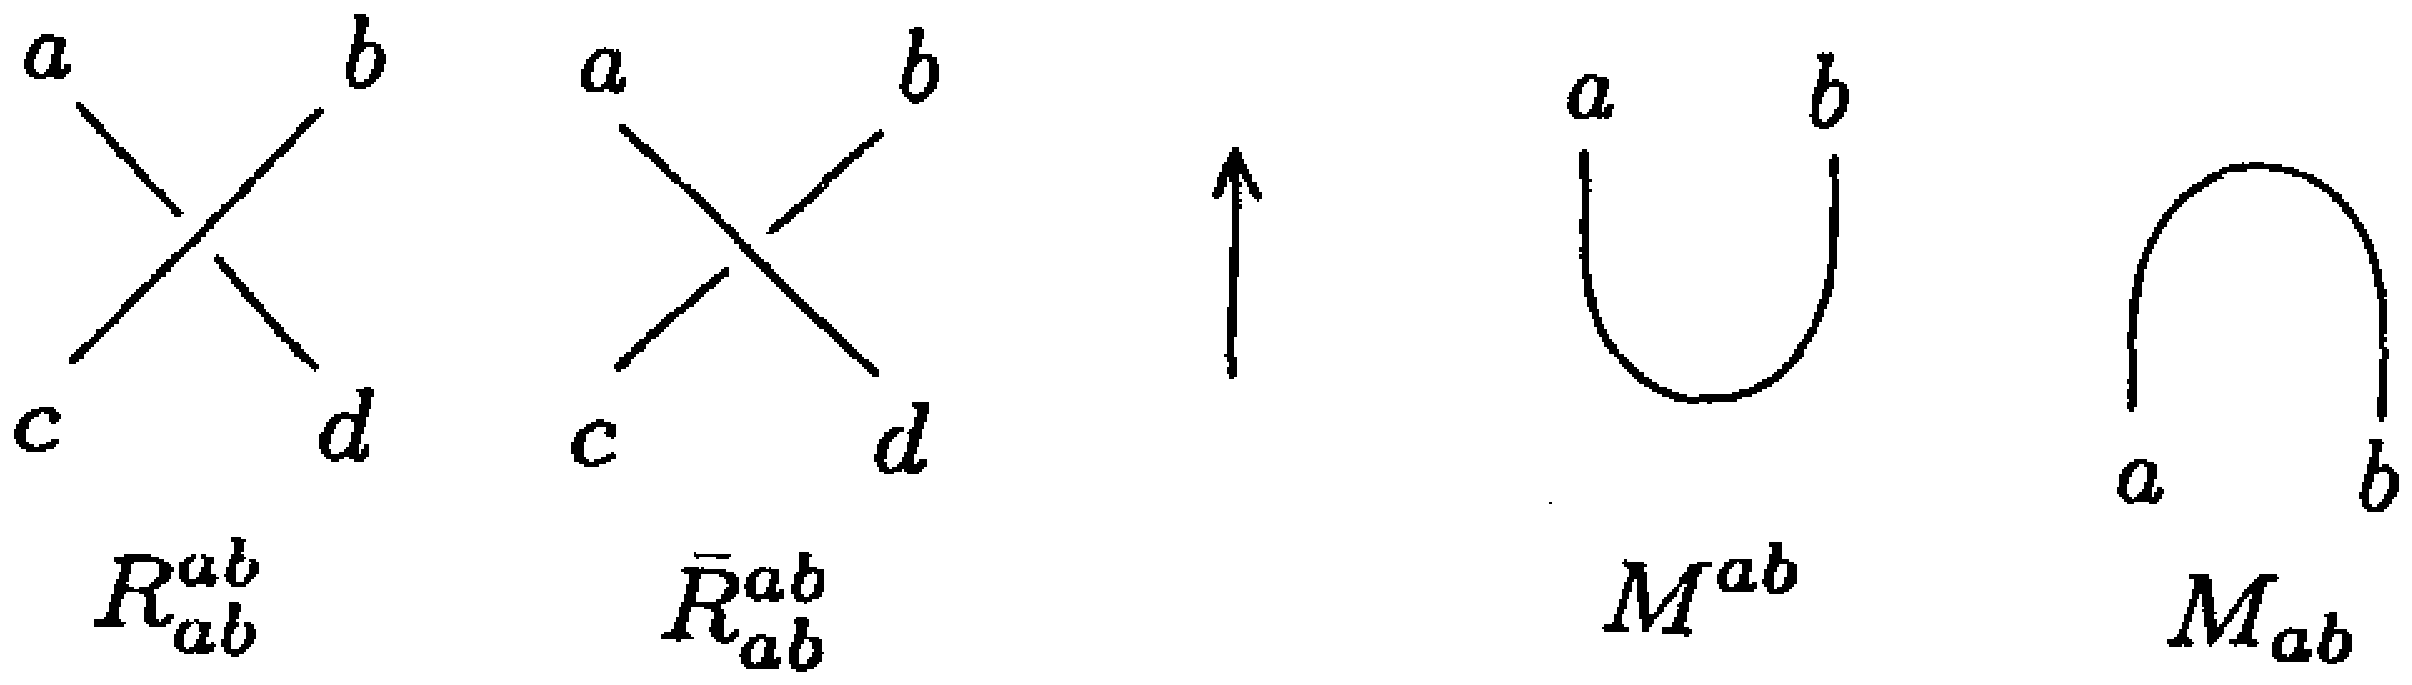
\includegraphics[width=0.86\textwidth]{figures/figA8.png}
\figtitle{A.8}{$R$ 矩阵以及杯、帽矩阵的定义}
\end{figure}

通过
\[
\tau(D)=\Tr[\eta\otimes\eta\otimes\cdots\otimes\eta\,\rho_n(B)]
\]
来定义\emph{Markov 迹}，其中 $\rho$ 是由 Yang--Baxter 方程的解 $R$ 所得到的表示，而
\[
\eta_a^b=M_{ai}M^{bi}.
\]

考虑由下式给出的显式解 $R$：
\[
R_{cd}^{ab}=AM^{ab}M_{cd}+A^{-1}\delta_c^a\delta_d^b,
\]

% [Tutor Note: 这里之所以要用「Markov 迹」而不是普通的矩阵迹，是因为普通迹只对共轭（第一种 Markov 变换）不变，对乘 $\sigma_{n+1}^{\pm 1}$ 却不行；把每个因子用 $\eta$（即杯—帽矩阵的复合 $\eta_a^b=M_{ai}M^{bi}$，几何上就是「把一根股弯回来」）缠接起来，才能让稳定化只带来一个常数因子。这也解释了前一处 Markov 性质里那个常数 $A$ 的来源：$A$ 是杯/帽与交叉矩阵的相对权重。]

% [原文 p.285]

\begin{figure}[htbp]
\centering
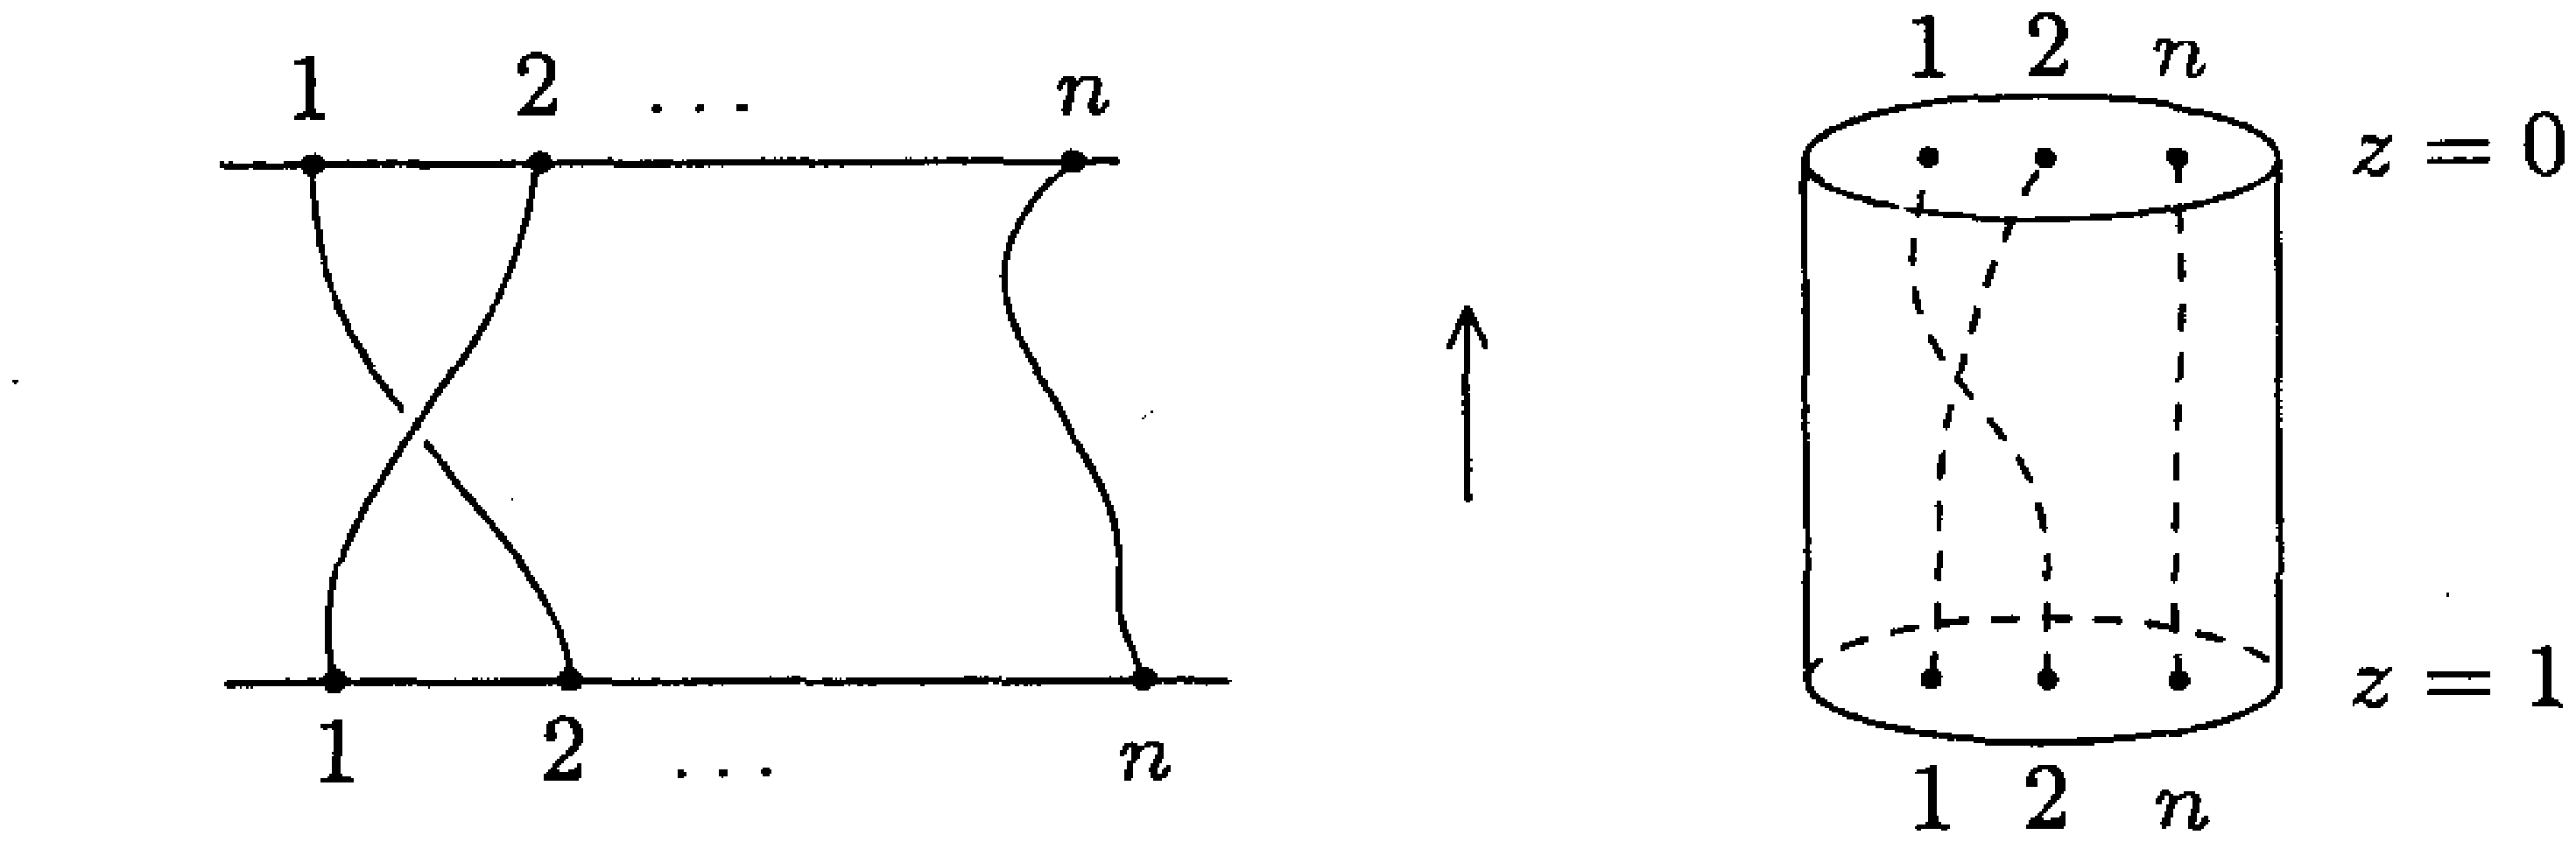
\includegraphics[width=0.92\textwidth]{figures/figA9.png}
\figtitle{A.9}{平面上闭辫的图；柱体中的闭辫}
\end{figure}

% [Tutor Note: 原书图 A.9 右半把柱体的上底标为 $z=0$、下底标为 $z=1$，与正文「$n$ 辫的起点在底面 $z=0$、终点在顶面 $z=1$，且 $Q_i$ 在 $P_i$ 正上方」正好相反；按正文，$z$ 增大应向上，故 $z=0$ 在下、$z=1$ 在上。图内标注照录原书，正文定义才是定论。]

\noindent 其中 $i^2=-1$，矩阵 $M$ 形如
\[
M=\begin{pmatrix}0&iA\\-iA^{-1}&0\end{pmatrix},
\]
指标集为 $I=(+,-)$。此处所论闭辫 $B$ 的图 $D$ 按无向着处理。但 $D$ 有一个由 $(x,z)$ 平面内 $z$ 轴方向所决定的自然定向。由此得到上面讨论过的 Kauffman--Jones 多项式的公式
\[
J(A^4,A^{-4})=(-A)^{-3w(D)}\tau(D).
\]

在有向图的情形，有一个由下式给出的显式解 $R$：
\[
R_{cd}^{ab}=\bigl((q-q^{-1})[a<b]+q[a=b]\bigr)\delta_c^a\delta_d^b+[a\ne b]\delta_d^a\delta_c^b,
\]
其中 $[P]$ 当命题 $P$ 为真时定义为 $1$、为假时定义为 $0$，指标集为 $I=I_n=(-n,-n+2,\dots,n)$。相应的解 $\bar R$ 可在此公式中把 $q$ 换成 $q^{-1}$、把 $a,b$ 换成 $-a,-b$ 而得到。这些 Yang--Baxter 解给出给定纽结或链环（其图 $D$ 有向）的如下拓扑不变量：
\[
P_D^{(n)}=\bigl(q^{(n+1)}\bigr)^{-w(D)}\langle D\|R,\bar R\rangle.
\]

于是 HOMFLY 多项式可通过取基数为 $n+1$ 的指标集 $I$（其中 $n\ge 1$）并作代换 $y=q^{n+1}$ 而得到。$n=1$ 时，代换 $q=t^{1/2}$ 给出 Jones 多项式。注意代换 $q=1$ 不给出任何新信息。

现在考虑缠结（tangles），即位于带域 $0\le z\le 1$ 中、带一个入边与一个出边的有向图 $D_1$，其两端分别落在直线 $z=0$ 与 $z=1$ 上。对指标集 $I=(-,+)$，我们总是把入边与出边都标以指标 $+$。于是，把平面内闭有向图 $D$ 沿一条（任意选定的）外部边剪开，便得到 $D$ 的 Alexander 多项式。

% [原文 p.286]

仿照 Jaeger 与 Kauffman 的做法，可以从如下 $R$ 矩阵得到 Alexander 多项式：取指标集 $I=(+1,-1)$，令
\[
R=(q-q^{-1})X_{+-}+qX_{++}-q^{-1}X_{--}+Y,
\]
然后把 $q$ 换成 $q^{-1}$、把 $X_{+-}$ 换成 $X_{-+}$，便得到 $\bar R$；这里张量 $X_{sp}$ 由
\[
(X_{sp})_{cd}^{ab}=
\begin{cases}
1, & \text{若 } a=c=s \text{ 且 } b=d=p,\\
0, & \text{其他情形},
\end{cases}
\]
给出，而张量 $Y$ 由
\[
Y_{cd}^{ab}=[a\ne b]\delta_d^a\delta_c^b
\]
给出，其中 $a,b,c,d=\pm1$。

Alexander 多项式也可以由辫群在若干个一维空间 $\R_i=\R$ 的直和上的「Burau 表示」得到：
\[
\rho(\sigma_i)=
\begin{bmatrix}
1&0&0\\
0&T&0\\
0&0&1
\end{bmatrix};
\]
这里 $1$ 表示任意阶的单位矩阵，而 $T$ 是 $2\times2$ 矩阵
\[
T=\begin{bmatrix}0&t\\1&(1-t)\end{bmatrix},
\]
它作用在 $\R_i\oplus\R_{i+1}$ 上。于是 Alexander 多项式由
\[
A_{D_a}=(\det)^*(\rho(a)-1_n)
\]
给出，其中 $D_a$ 是由辫 $a$ 得到的相应闭辫，而 $(\det)^*$ 表示矩阵 $\rho(a)-1_n$ 的任一 $(n-1)$ 阶子式。这样得到的 Alexander 多项式在相差 $\pm t^m$（$m$ 为任意整数）的意义下是良定的。

值得指出线性变换 $M$ 的外幂的如下有趣恒等式：
\[
\det(M-\lambda 1_n)=\sum_{j=0}^{j=n}\Tr\bigl((-\lambda)^k\Lambda^k M\bigr);
\]
% [Tutor Note: 原书此式求和指标前后不一致：上下限写作 $j=0$ 至 $j=n$，而通项里用的却是 $k$。按外幂的标准恒等式（特征多项式的系数恰由各阶外幂的迹给出），求和指标应为 $k$，即 $\det(M-\lambda 1_n)=\sum_{k=0}^{n}(-\lambda)^k\Tr(\Lambda^k M)$。此处照录原书，读者按 $k$ 读即可。]
这导致一个（非 Markov 的）迹，并导致与上面用缠结构造 Alexander 多项式时所用者本质上等价的 Yang--Baxter 解 $R$、$\bar R$。

在现代纽结与 3 维流形理论中，有三个很好用的代数对象：Hecke 代数、Temperley--Lieb（或 Jones）代数，以及 Birman--Wenzl 代数。它们定义如下：

% [原文 p.287]

\emph{Hecke 代数}由元素 $\sigma_i$（$i\in\Z$）生成，它们满足辫关系（见上），以及形如
\[
\sigma_i-\sigma_{i-1}=z
\]
的关系，其中 $z$ 可以是一个数，也可以取在代数的中心里。

% [Tutor Note: 原书此处把 $z$ 前的下标印作 $i-1$，但 Hecke 代数的标准关系是 $\sigma_i-\sigma_i^{-1}=z$（等价于 $(\sigma_i-q)(\sigma_i+1)=0$ 型的关系）：辫群的生成元之间并不存在 $\sigma_i-\sigma_{i-1}=z$ 这样的关系，而同一页下文的 Birman--Wenzl 代数明确写作 $\sigma_i-\sigma_i^{-1}=z(v_i-1)$。故此处应为上标 $-1$ 误排成下标 $i-1$；正文照录原书，读者按 $\sigma_i-\sigma_i^{-1}=z$ 读即可。]

\emph{Temperley--Lieb 代数}（TL）定义在环 $\Z[A,A^{-1}]$ 上，由生成元 $v_i$（$i\in\Z$）给出，满足关系
\begin{gather*}
v_iv_j=v_jv_i,\qquad |i-j|>1,\\
v_iv_{i\pm1}v_i=v_i.
\end{gather*}
这里 $A$ 可以取某个数。有一个与之相伴的\emph{抽象迹}，即线性映射
\[
f:TL\to\Z[A,A^{-1}],
\]
满足对一切 $u,v$ 有 $f(uv)=f(vu)$。还应注意，一般地可得到辫群在 TL 中的一个表示
\[
\rho(\sigma_i)=av_i+b,
\]
其中 $a,b$ 为适当的数。

\emph{Jones 代数}与 TL 相同，只是改用生成元 $e_i=\delta^{-1}v_i$ 来给出，其中 $-\delta=A^2+A^{-2}$，而 $e_i$ 是投影：$e_i^2=e_i$。

\emph{Birman--Wenzl 代数}也由 $\sigma_i$ 生成，并附加关系
\[
\sigma_i-\sigma_i^{-1}=z(v_i-1).
\]
容易看出，它可实现为 TL 的子代数。

由辫与 Yang--Baxter 方程出发，Drinfeld、Jimbo、Sklyanin、Kulish、Faddeev、Takhtadjan、Reshetikhin、Voronovich 等人构造出了「量子群」理论。这套理论对 Yang--Baxter 方程那些最熟悉的解的行为作了令人愉快的系统化：它用某些代数来组织这些解，而 Drinfeld 证明，这些代数就是装备了一种称为「量子双」的漂亮附加结构的 Hopf 代数。（用他的术语，这是半单 Lie 代数的包络代数的「量子形变」。）

这一醒目的术语，其实仅仅来自如下性质：在一阶近似下，这种形变由 Lie 群上某个 Poisson 括号所决定，因此从表面上看，它似乎表示把群作为相空间来作的某种量子化。（这类括号此前曾在孤子理论中某些（并非全部）可积模型里出现过。）然而这一程序实际上并不表示对群或 Lie 代数作了任何量子化——如果我们把群或 Lie 代数看作度量某个待量子化物理系统的对称性的对象的话。

若干例子表明，这一非常吸引人的构造，在某种微妙而非平凡的意义上，更像是「离散化」而不是「量子化」（后者是按该词在分析中对称性语境下的通常用法；事实上类似「解析计算的 $q$-形变」这样的非平凡事物可以追溯到 19 世纪）。然而「量子群」这个说法听起来很了不起，给它平添了一层或许有些虚妄的兴奋气氛。（Landau 研究所一位本身发现过许多 Yang--Baxter 方程非平凡解的一流量子物理学家，在 1980 年代末曾对本书作者说，他「不知道『量子群』是什么意思，但听起来非常吸引人」。不过看来他自己其实早已把量子群用于磁场中 Schrödinger 算子的离散化了。）

% [原文 p.288]

看来量子群这一技巧有望用来改进上述多项式不变量的某些已知结果。但迄今为止，沿着这条路线除了把已知结果系统化之外，还没有取得任何成果，尽管这一途径看起来仍然很有前途。

Jones 多项式引出了若干漂亮的新结果。其中之一如下。19 世纪末，物理学家 Tait 循 Maxwell 或 Thomson（开尔文勋爵）的某个建议开始研究纽结。他编纂了最简单非平凡纽结的表，并特别注意到表中「交错」纽结的各种性质，即那些沿纽结的有向图行走时下穿与上穿交替出现的纽结。1980 年代末，Kauffman 与 Murasugi 用 Jones 多项式证明：只要对应的有向图不可约——即它不能由两个非平凡图用一对互不相交的线段连接而成（见图 A.10）——交叉数就是该纽结的拓扑不变量。（事实上，不可约交错图的交叉数等于 Jones 多项式 $J(t,t^{-1})$ 中出现的 $t$ 的最高次幂与最低次幂之差。）

% [Tutor Note: 原书把开尔文勋爵的姓排作 Thompson，通行的拼法是 Thomson（William Thomson，1824--1907）；正文按通行拼法写作 Thomson，读者不必以为另有一人。Tait 即 P. G. Tait。又，原书此处的 Jones 多项式印成 $J(t,t^{-1})$，把 $t$ 与 $t^{-1}$ 并列成两个自变量，实际只是提醒该多项式是 $t$ 的 Laurent 多项式。]

\begin{figure}[htbp]
\centering
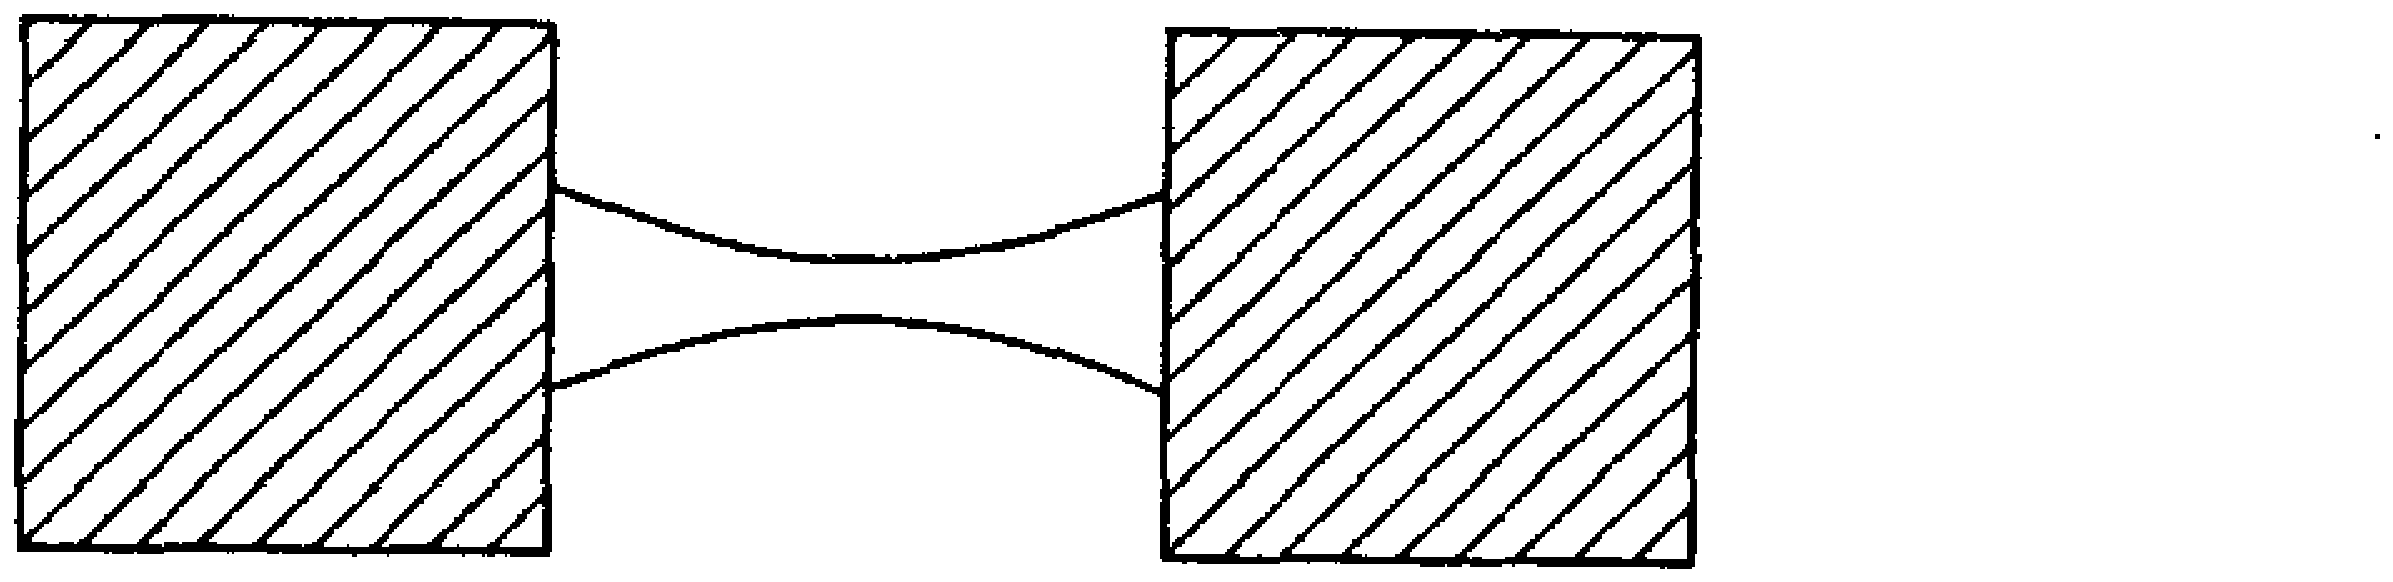
\includegraphics[width=0.78\textwidth]{figures/figA10.png}
\figtitle{A.10}{可约图}
\end{figure}

尽管这从来不被看作纽结理论的一个重大问题，但古典拓扑学的方法似乎不足以解决它，这一点却是有意义的。这（以及其他结果）证明了 Jones 多项式的发现具有何等重大的意义。

% [原文 p.289]

顺便再提 Alexander 多项式的一个早已为人所知的好性质：对\emph{带状纽结}（ribbon knot，即作为 $\R^3$ 中浸入 2-圆盘的边界者）存在多项式 $f(t)$，使
\[
A(t,t^{-1})=f(t)f(t^{-1}).
\]

\section{Vassiliev 不变量}

\takeaway{Vassiliev 不变量把多项式不变量的可加性解释成「对奇点的导数」：$k$ 阶不变量由跨过 $k$ 重自交点的跳跃给出，而 $k$ 阶不变量就是第 $(k+1)$ 阶导数为零者，据此可把纽结不变量按「阶」分层。}

Alexander 多项式与 Jones 多项式的可加性质，用「Vassiliev 不变量」的语言有一个非常吸引人的解释。这一不变量理论大约出现在最近 5 年间；其主要阐述者有 V. Vassiliev、D. Bar--Natan、J. Birman、X-S. Lin、M. Kontzevich。

考虑圆周 $S^1$ 在 $\R^3$ 中的一切浸入所构成的空间 $F_k$。这里所论的每个浸入（记作 $G_k$）都要求其像恰有 $k$ 个二重点（交叉点）$P_i,\bar P_i\in S^1$（$i=1,\dots,k$），且像曲线在每个这样的点处都与自身横截相交。把像在某个这样的交点附近作扰动，便得到一对浸入 $G_{k-1}^+,G_{k-1}^-$，各含 $(k-1)$ 个交叉点，因而属于空间 $F_{k-1}$（见图 A.11）。

\begin{figure}[htbp]
\centering
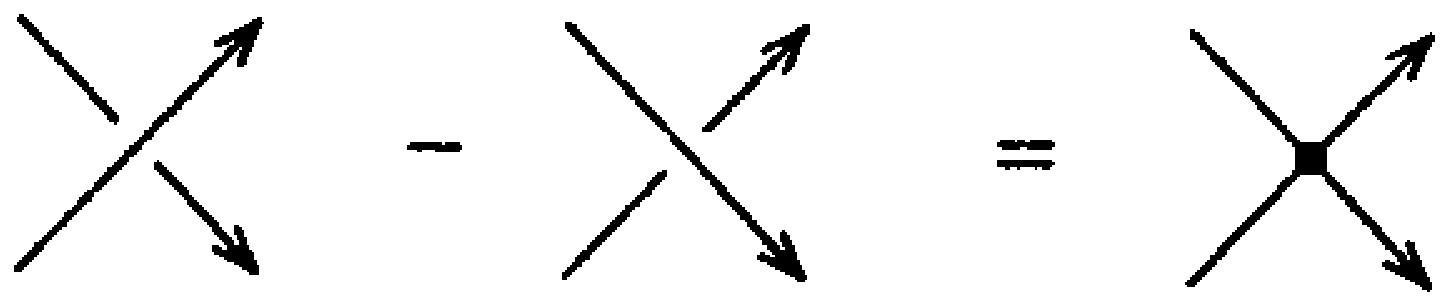
\includegraphics[width=0.62\textwidth]{figures/figA11.png}
\figtitle{A.11}{Vassiliev 导数的定义}
\end{figure}

% [Tutor Note: $P_i,\bar P_i\in S^1$ 是同一个二重点在圆周 $S^1$ 上的两个原像，故一对字母才给出一个交叉点；把像在交点附近扰动，本质上就是把「一个二重点」换成「两个一重点之间的一个小弧」，图上第三个（画了黑点的）交叉即代表被求导的那处奇点。]

考虑空间 $F_k$ 的一个拓扑不变量 $f_k$，即从 $F_k$ 的分量集合到某个交换群 $A$ 的任意函数：
\[
f_k:\pi_0(F_k)\to A.
\]
特别地，当 $k=0$ 时我们恰好得到纽结的拓扑不变量。我们把这样的不变量 $f_k$ 称为某个不变量 $f_{k-1}$ 的 \emph{Vassiliev 导数}，如果下列等式成立：
\[
f_{k-1}(G_{k-1}^+)-f_{k-1}(G_{k-1}^-)=f_k(G_k).
\]
纽结的一个拓扑不变量若其第 $(k+1)$ 阶 Vassiliev 导数为零，就称为 \emph{Vassiliev $k$-不变量}。

由 Bar--Natan 的一个结果，Alexander 多项式的所有系数都是 Vassiliev 不变量。几年前 Bar--Natan、Lin 与 Birman 还从 HOMFLY 多项式的可加性质推出：在作代换
\[
y=\exp(Nx),\qquad x=\exp\Bigl(\frac z2\Bigr)-\exp\Bigl(-\frac z2\Bigr),
\]
之后，HOMFLY 多项式作为 $z$ 的幂级数的系数都是 Vassiliev 不变量。

% [原文 p.290]

Kontzevich 有一个吸引人的公式，用多重积分解析地表示出所有 Vassiliev 不变量，前提是纽结或链环的图带有某个通有的 Morse 函数（例如把平面图投影到 $y$ 轴上）。

所有可能的 Vassiliev 不变量还有纯组合的刻画，不过它在目前对于计算具体不变量而言是不实用的。（事实上，除了上述纽结的 Alexander 与 HOMFLY 多项式的系数之外，目前还不知道任何具体的 Vassiliev 不变量。）

\begin{figure}[htbp]
\centering
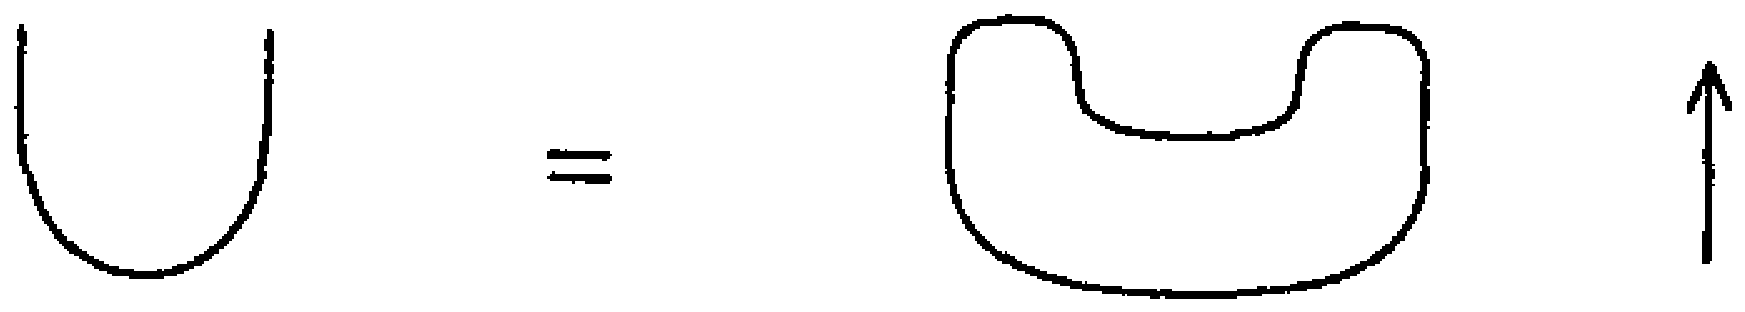
\includegraphics[width=0.60\textwidth]{figures/figA12.png}
\figtitle{A.12}{图 $U$}
\end{figure}

这一组合描述如下。\emph{弦图}（chord diagram）定义为一个圆周，上面标有 $2k$ 个互不相同的点 $P_j,Q_j$（$j=1,2,\dots,k$）。（事实上，这里只有这些点沿圆周的循环次序是有意义的。）现在我们对由所有弦图（含 $2k$ 个点）自由生成的自由交换群施加如下关系：

\begin{enumerate}
\item 若弦图含有一对点 $P_j,Q_j$，它与任何其他对都「不相链」，即对任何 $i$，只要在绕圆周的循环次序中有 $P_j<P_i<Q_j$，就也有 $P_j<Q_i<Q_j$，则该弦图被置为零。

\item 任给 $(k-2)$ 对点 $P_j,Q_j$（$j=1,\dots,k-2$）以及圆周上另外三个互不相同的点 $A_1,A_2,A_3$，可以如下构造一个含 $2k$ 个点的弦图：先把 $A_1,A_2,A_3$ 中的某一点换成紧邻它的两个点（都靠近所选定的 $A_i$），标号为 $P_{k-1},P_k$，再把剩下的两个点之一标为 $Q_{k-1}$、另一个标为 $Q_k$；由于这一重新标号可以有两种不同的做法，这样得到的弦图有两个，记为 $C_+$ 与 $C_-$；于是，若首先选中的点是 $A_1$，则 $C_+$ 与 $C_-$ 由
\[
\begin{aligned}
C_+:&\quad A_2=Q_{k-1},\quad A_3=Q_k,\\
C_-:&\quad A_2=Q_k,\quad A_3=Q_{k-1}
\end{aligned}
\]
给出。
\end{enumerate}

% [Tutor Note: 弦图记录的是「$k$ 个二重点的原像配对」：圆周上 $2k$ 个点两两配成 $k$ 对 $P_j,Q_j$，每一对就是从奇点集里取出的一个交叉点在 $S^1$ 上的两个原像。关系 1 说的是：若某一对的整个弧段里不含别的对，则这个弦图代表零（对应「可约去」的奇点）；关系 2 则是把三重点拆成二重点时的两种次序，差 $C_+-C_-$ 与先选哪个点无关，正对应 Vassiliev 导数的高阶相容性。]

于是再施加关系，以保证差 $C_+-C_-$ 与在 $A_1,A_2,A_3$ 这一点三元组中先选哪一点无关。

这样得到的商群 $B_k$ 便把所有 Vassiliev $k$-不变量都编码于其中。

% [原文 p.291]

分次直和
\[
B=\sum_{k\ge0}B_k
\]
可以通过沿与标记点不交的弧作弦图的连通和来定义乘法，从而被赋予分次 Hopf 环的结构。（这个乘法之所以良定，是上述 $B_k$ 的定义关系的一个推论。）

现在叙述 Kontzevich 的公式；由它容易推出，$B_k$ 的每个元素确实对应一个 Vassiliev 不变量。设 $K$ 是 $\R^3$ 中的定向纽结，由坐标 $z=z(t)(=x(t)+iy(t))$、$t$ 给出。（这里 $t$ 可以看作 $K$ 上的一个通有 Morse 函数。）考虑如下求和（即「Kniznik--Zamolodchikov 单值性」）：
\[
Z(K)=\sum_m\frac{1}{(2\pi i)^m}\int\cdots\int_{\substack{t_{\min}<t_1\cdots t_n<t_{\max}\\ \|\ AS[\text{点对 } z_j,z_j^1]}}(-1)^{N\downarrow}\prod_j d\log(z_j-z_j^1)\,D_N;
\]
这里积分是对变量 $t_s$ 取的。对 $t_s$ 的每个值，有纽结 $K$ 上的点集 $(z(t_s),t_s)$，并从此集里选取 $m_s$ 对点（选取由 $AS$ 标出）
\[
(z_j(t_s),t_s),\quad (z_j^1(t_s),t_s),\qquad j=1,\dots,m_s,
\]
其中 $\sum_s m_s=m$。相应的弦图就取作带有这一族点对的圆周。记号 $N\downarrow$ 表示相对于 $t$ 的下行弦的数目。记 $s=s_K$ 为纽结 $K$ 的极小点的个数，并令 $\gamma:=Z(U)$，其中 $U$ 如图 A.12 所示；于是有 Kontzevich 的如下公式：
\[
\gamma^{-s}Z(K)\ \text{是拓扑（Vassiliev）不变量}.
\]

% [Tutor Note: 原书此式有两处不易自明：其一，末尾的 $D_N$ 含义不明（疑为排版残留或某种测度记号），此处照录原书，不影响对公式其余部分的理解；其二，积分区域的条件写作 $t_{\min}<t_1\cdots t_n<t_{\max}$，意思是 $t$ 参数落在极小点与极大点之间、且各 $t_s$ 依序排列；求和指标原用 $m$，条件里却写 $n$，也是原书记法。]

\section{3 维流形的新拓扑不变量与拓扑量子场论}

\takeaway{Witten 把 Reidemeister--Ray--Singer 挠率的 Schwarz 表示推广为 Chern--Simons 型泛函积分，由此给出 3 维流形的新拓扑不变量，即拓扑量子场论的配分函数 $Z(M^3)$；它与量子群、Jones 多项式同出一源。}

现在我们来描述这些想法在研究 3 维流形的新拓扑不变量方面的一些应用。这些不变量由 Witten 发现，是 Reidemeister--Ray--Singer 挠率的 Schwarz 表示的自然非交换推广，其形式是「Chern--Simons」型泛函积分，即在规范等价类的空间上的一个多值作用泛函，而该空间是 Yang--Mills 场的空间（亦即主 $G$-丛上的微分几何联络，其中 $G$ 是任意紧 Lie 群，例如 $G=SU_2$）。

存在一个定义在 3 维流形类上的、如下形式的「配分函数」（前提是它有意义）：

\[
Z(M^3)=\int DA(x)\exp\{ikS(A)\},\qquad i^2=-1.
\]

% CHUNK appb DONE
